\chapter{Analisi delle connessioni di un singolo nodo}



\vspace*{1cm}

\section{Motivazioni}
Abbiamo visto nei capitoli precedenti come pu\`o essere utilizzata la tecnologia introdotta da Satoshi Nakamoto, e analizzato anche al livello pi\`u tecnico le parti fondamentali che costituiscono l'ecosistema Bitcoin.\\
In questo, e nel successivo capitolo voglio focalizzarmi sulla topologia della rete \textit{peer-to-peer} sulla quale si poggia Bitcoin.
Si \`e gi\`a accennato il fatto che la topologia di tale rete \`e deliberatamente tenuta nascosta, ma quali sono le motivazione principali del perch\`e debba essere segreta?
La conoscenza della topologia della rete non deve essere per forza considerata una minaccia o una vulnerabilit\`a, sebbene potrebbe comunque essere utilizzata in modo inappropiato da parte di hacker che potrebbero creare attacchi che hanno come bersaglio la rete stessa o rendere note le identit\`a degli \textit{user}, sappiamo bene che l'anonaminit\`a \`e una delle caratteristiche pi\`u apprezzate della tecnologia Bitcoin.
Un esempio di attacchi di questa tipo \`e l' \textit{eclipse attack}, basato su un network decentralizzato in cui chi attacca cerca di isolare uno specifico \textit{user} anzich\`e attaccare l'intera rete, e ovviamente conoscendo la topologia della stessa risulterebbe molto pi\`u facile identificare quali siano i nodi con meno connessioni e quindi pi\`u isolati.
Uno studio sulla topologia della rete potrebbe comunque rivelare delle caratteristiche interessanti riguardanti la stessa, si potrebbe vedere in che misura la rete sia veramente decentralizzata identificando \textit{supernodi}, \textit{nodi ponte}, \textit{potenziali punti di rottura,} ecc.. 
Lo studio della topologia della rete di Bitcoin \`e stato argomento di studio da parte di vari gruppi di ricerca, ognuno dei quali ha affrontato il problema di inferire le connessioni del network in maniera e con tecniche differenti.
La tecnica mostrata nel paper \cite{delgado2018txprobe} si basa fortemente sul monitoraggio delle \textit{pool} delle transazioni orfane e su come queste vengano propagate all'interno del network Bitcoin. Un approccio differente \`e invece quello descritto in \cite{miller2015discovering} dove le connessioni tra i nodi vengono identificate attraverso l'analisi dei \textit{timestamp} i quali vengono aggiornati continuamente quando i nodi della rete si scambiano messaggi. Infine vorrei citare il \cite{neudecker2016timing} nel quale viene mostrato come inferire la topologia della rete Bitcoin facendo osservazioni e comparazioni tra le informazioni riguardo al \textit{delay} di propagazione della rete Bitcoin e il \textit{delay} di propagazione di un modello matematico scelto come confronto. \\
In questa tesi avremo un obiettivo meno ambizioso, andremo ad analizzare coma cambia la rete dal punto di vista di un singolo nodo. Per questo esperimento si \`e installato un \textit{full node} che monitoreremo periodicamente per ricavare dei dati circa lo stato delle sue connessioni con altri \textit{peers}, si andr\`a poi a fare un analisi dei dati cosi raccolti, attraverso un programma scritto in python che evidenzier\`a varie caratteristiche derivate dall'elaborazione di questi dati come ad esempio la percentuale dei nodi che rimangono connessi dall'inizio alla fine della monitorizzazione, la probabilit\`a in media che una connessione "crolli", metter\`a in risalto inoltre quei nodi che sono rimasti connessi per pi\`u tempo poich\`e potrebbero essere nodi stabili della rete, sar\`a mostrato con un grafico a barre per ogni \textit{peer} (identificato dall'indirizzo IP) la percentuale di tempo che \`e rimasto in connessione con il nostro \textit{full node} e vederemo se l'analisi di differenti monitorizzazioni produrranno risultati simili.




\section{Descrizione dell'applicativo}
L'applicativo consiste nel richiamo periodico del comando \textit{bitcoin-cli getpeerinfo} da parte di un \textit{full node} in nostro possesso. Questo comando ritorna alcune informazioni riguardanti le connessioni del nodo verso altri nodi della rete, possiamo vedere un esempio nella figura \textit{3.1}.
\begin{figure}[H]
\begin{center}
   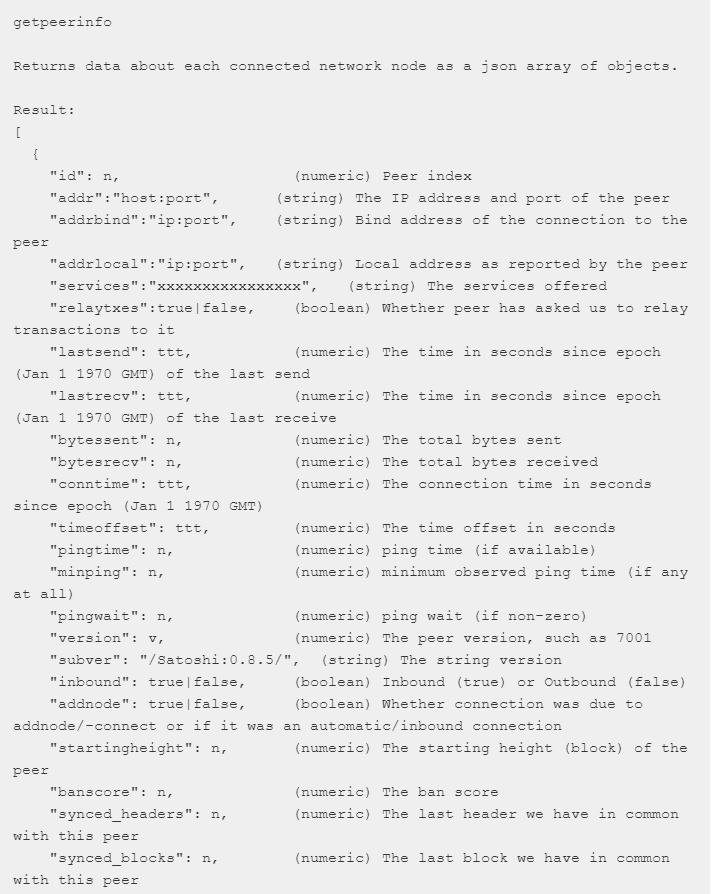
\includegraphics[width=0.555\textwidth]{imgs/getpeerinfo.png}
   \caption{https://bitcoincore.org/en/doc/0.16.0/rpc/network/getpeerinfo/}
   \end{center}
   \hfill
\end{figure}
Lanciando pi\`u volte il comando appena descritto potremmo ricavare dati utili da elaborare con lo scopo di capire il comportamento del nostro nodo e i suoi vicini all'interno del network.\\
L'applicativo consiste in due programmi scritti in python, \textit{raccolta\_dati\_csv.py} e \textit{analisi\_dati\_csv.py}.
Il primo serve appunto per raccogliere informazioni circa il nostro \textit{full node}, quando viene richiamato questo richiede un parametro, \textit{param1}, che indica il nome del file che il programma andr\`a a creare per salvare i dati raccolti (si veda figura \textit{3.2}).
\begin{figure}[htb]
\begin{center}
   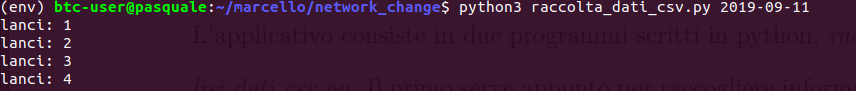
\includegraphics[width=0.755\textwidth]{imgs/raccolta_dati_csv.png}
   \caption{Esempio lancio del programma raccolta\_dati.py}
   \end{center}
   \hfill
\end{figure}
L'intervallo di tempo tra due "lanci" consecutivi \`e di 5 minuti, il programma raccoglier\`a dati ad oltranza finch\`e non verr\`a fermato. Ogni ora comuqnue sar\`a creato un file di backup dei dati fino a quel momento ottenuti.
I file creati saranno dei \textit{CSV}, in cui in ogni riga, il primo valore indicher\`a il timestamp, mentre gli altri, saranno la lista diindirizzi  IP che erano connessi al nostro nodo in quel preciso momento.
Come gi\`a accennato i risultati saranno salvati in una cartella identificata dal nome \textit{param1}, all'interno della quale troveremo il file dei dati effettivi denominato \textit{param1.txt}, inoltre sar\`a creata anche un'altra cartella con all'interno un medesimo file di backup.\\
Una volta recuperati questi dati  (si veda figura \textit{3.3}) 
\begin{figure}[htb]
\begin{center}
   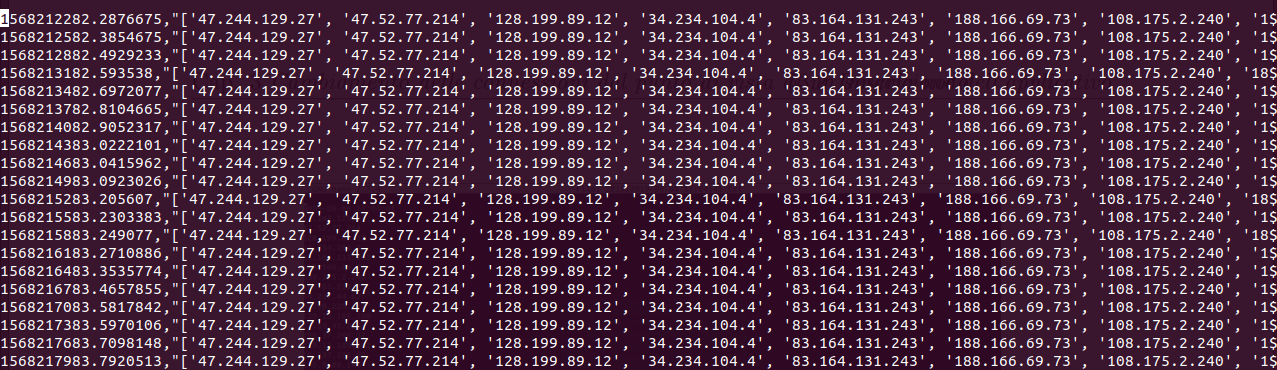
\includegraphics[width=0.755\textwidth]{imgs/dati_csv.png}
   \caption{Esempio dati raccolti.py}
   \end{center}
   \hfill
\end{figure}
dalla monitorizzazione del \textit{full node}, il programma \textit{analisi\_dati\_csv.py} li andr\`a ad elaborare per estrapolarne alcune statistiche. Questo secondo programma dovr\`a essere richiamato con un parametro che indichi il \textit{path} del file di cui siamo interessati. (si veda figura \textit{3.4}).\\
\begin{figure}[htb]
\begin{center}
   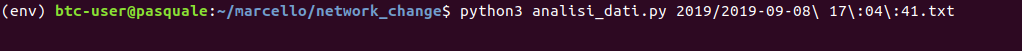
\includegraphics[width=0.755\textwidth]{imgs/analisi_dati.png}
   \caption{Esempio lancio del programma analisi\_dati.py}
   \end{center}
   \hfill
\end{figure}
Alla fine dell'elaborazione del programma saranno create tre cartelle: \textit{risultati\_param1, geolocate\_param1, e intervalli\_param1}.
Nella prima cartella troveremo un file con alcune statitistiche. Alle prime righe saranno identificati il giorno e l'orario in cui la monitorizzazione ha avuto inizio e quello in cui \`e terminata (si veda figura \textit{3.5}).
\begin{figure}[htb]
\begin{center}
   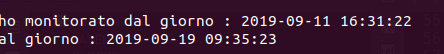
\includegraphics[width=0.755\textwidth]{imgs/tempo.png}
   \caption{Date di inizio e fine monitorizzazionr}
   \end{center}
   \hfill
\end{figure}
Dopo di ch\`e ci sar\`a una lista formata da tre valori: lancio - percentuale - numero di peer connessi(si veda figura \textit{3.6}).
\begin{figure}[htb]
\begin{center}
   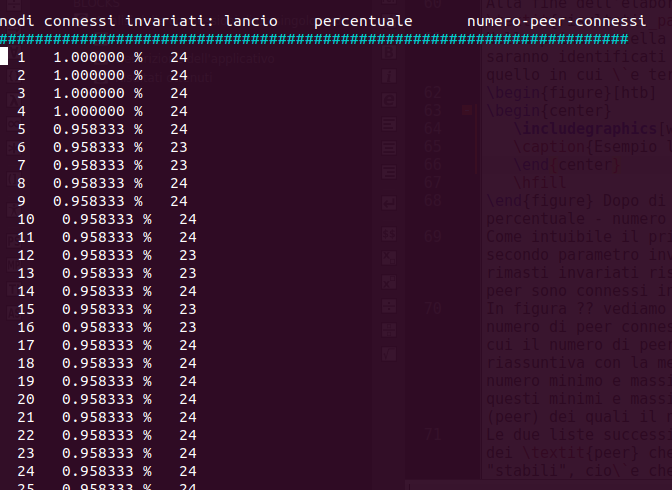
\includegraphics[width=0.755\textwidth]{imgs/lista3.png}
   \caption{Percentuale dei \textit{peer} invariati per ogni lancio}
   \end{center}
   \hfill
\end{figure}
Come intuibile il primo di questi valori indica il numero di lancio considerato, il secondo parametro invece indica quanti peer in percentuale in quel dato lancio sono rimasti invariati rispetto alla prima monitorizzazione, mentre l'ultimo indica quanti peer sono connessi in quel momento.
In figura \textit{3.7} vediamo una lista che indica i lanci in cui si \`e notato il massimo numero di peer connessi (in questo caso 24) e una lista che indica invece i lanci in cui il numero di peer connessi \`e stato minimo (in questo caso 22). Una tabella riassuntiva con la media di peer connessi ad ogni lancio, la relativa varianza, il numero minimo e massimo di peer connessi durante la monitorizzazione, e in quanti lanci questi minimi e massimi si sono verificati. Infine il numero totale di indirizzi IP (peer) dei quali il nostro \textit{full-node} \`e venuto a conoscienza.
Le due liste successive che vediamo sempre in figura contengono invece gli indirizzi dei \textit{peer} che si sono presentati con minor frequenza, e quelli che chiamiamo "stabili", cio\`e che sono sempre rimasti connessi.
\begin{figure}[htb]
\begin{center}
   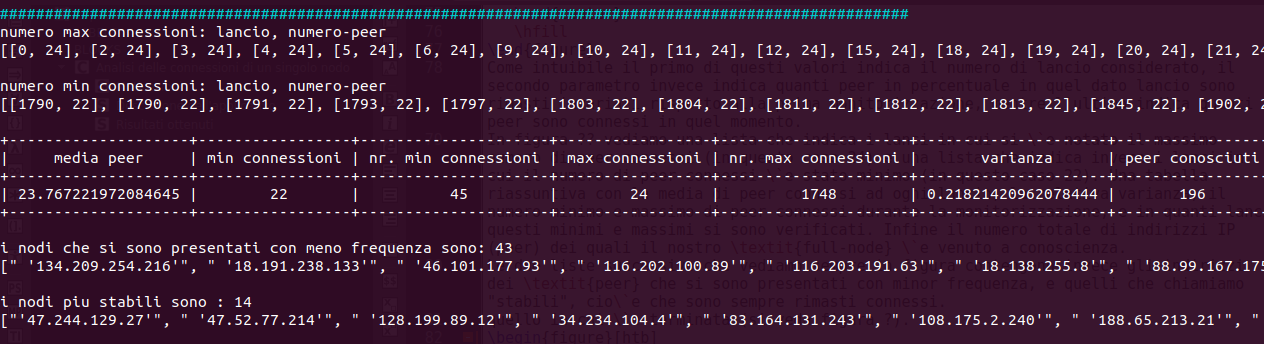
\includegraphics[width=1.000\textwidth]{imgs/tabella1.png}
   \caption{Statistiche sulle connessioni dei \textit{peer}}
   \end{center}
   \hfill
\end{figure}
Il programma mostrer\`a inoltre un rudimentale grafico a barre (figura \textit{3.8}) dove per ogni indirizzo IP ci sar\`a la percentuale di tempo per cui \`e rimasto connesso.
\begin{figure}[htb]
\begin{center}
   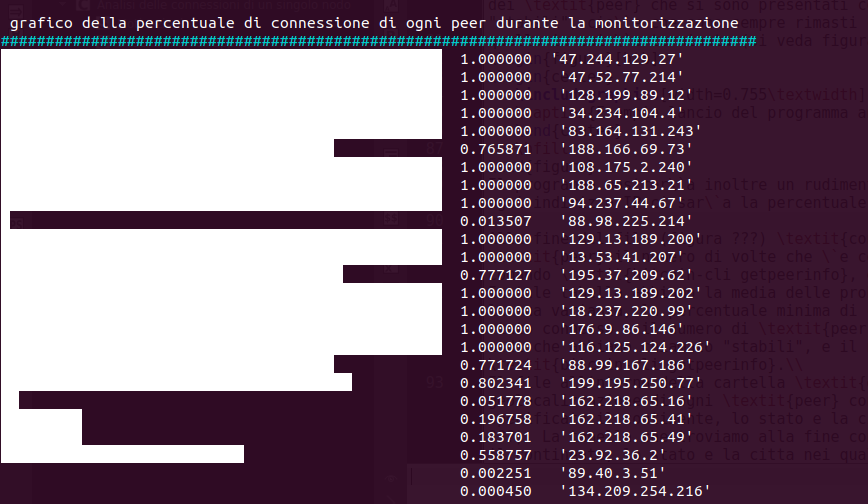
\includegraphics[width=0.755\textwidth]{imgs/grafico.png}
   \caption{Grafico a barre}
   \end{center}
   \hfill
\end{figure}
Alla fine del file (figura \textit{3.9}) \textit{connessioni peer} conterra per ogni \textit{peer} il numero di volte che \`e comparso durante la monitorizzazione del comando \textit{bitcoin-cli getpeerinfo}, e una tabella riassuntiva.
\begin{figure}[htb]
\begin{center}
   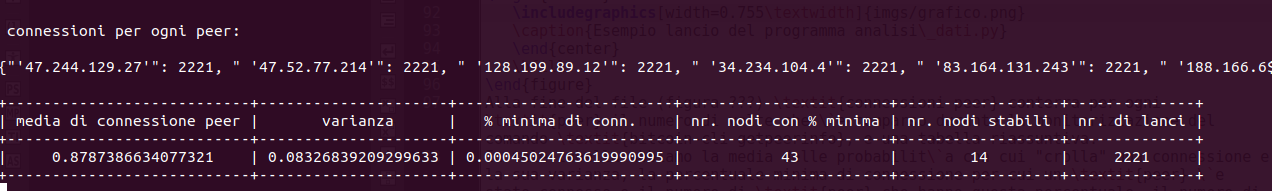
\includegraphics[width=0.755\textwidth]{imgs/tabella2.png}
   \caption{Statistiche sulla percentuale di connessione di ogni peer}
   \end{center}
   \hfill
\end{figure}
In tale tabella abbiamo la media delle probabilit\`a con cui "crolla" una connessione e la sua varianza, la percentuale minima di connessione per cui un \textit{peer} \`e stato connesso e il numero di \textit{peer} che hanno questa percentuale, il numero di nodi che abbiamo chiamato "stabili", e il numero di lanci totali del comando \textit{bitcoin-cli getpeerinfo}.\\
Il file all'nterno della cartella \textit{geolocate\_param1} contiene dati riguardo la geolocalizzazione di ogni \textit{peer} conosciuto. Per ogni indirizzo IP \`e specificato il continente, lo stato e la citt\`a in cui esso si trova (vedi figura \textit{3.10}).
\begin{figure}[htb]
\begin{center}
   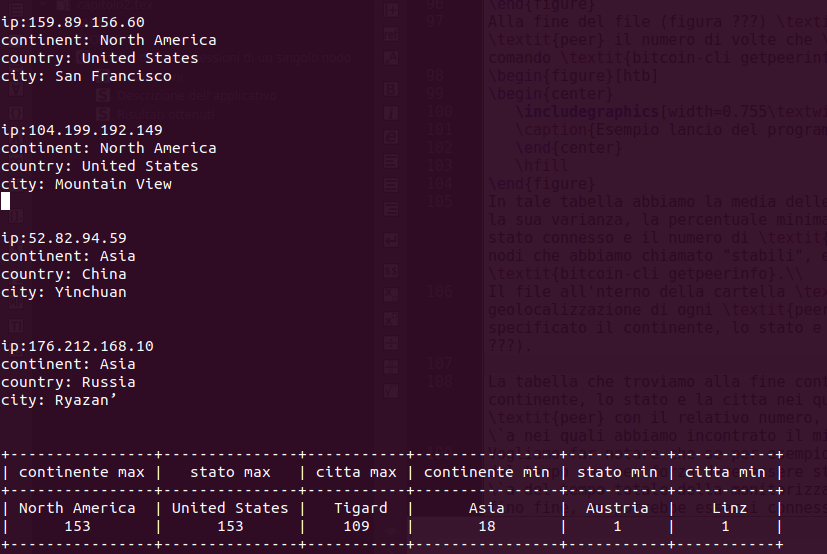
\includegraphics[width=0.755\textwidth]{imgs/geolocate.png}
   \caption{Geolocalizzazione dei \textit{peer}}
   \end{center}
   \hfill
\end{figure}
La tabella che troviamo alla fine contiene alcuni campi importanti tra i quali: il continente, lo stato e la citta nei quali abbiamo incontrato il maggior numero di \textit{peer} con il relativo numero, e analogamente il continente, lo stato e la citt\`a nei quali abbiamo incontrato il minor numero di \textit{peer}.
Vogliamo far notare che se per esempio un \textit{peer} \`e stato connesso per il 50\% del tempo non per forza deve essere stato connesso dall'inizio fino alla fine prima met\`a del tempo totale della monitorizzazione, oppure dall'inizio della seconda met\`a fino fine, ma potrebbe essersi connesso e riconesso pi\`u volte fino a totalizzare la percentuale prima indicata.
Per questo scopo nell'ultima cartella, \textit{intervalli\_param1}, per ogni \textit{peer} viene indicato l'intervallo di tempo in cui questo \`e stato connesso, nel caso quindi di connessioni discontinue, un indirizzo IP sar\`a affiancato da pi\`u intervalli di tempo (si veda figura \textit{3.11}).
\begin{figure}[htb]
\begin{center}
   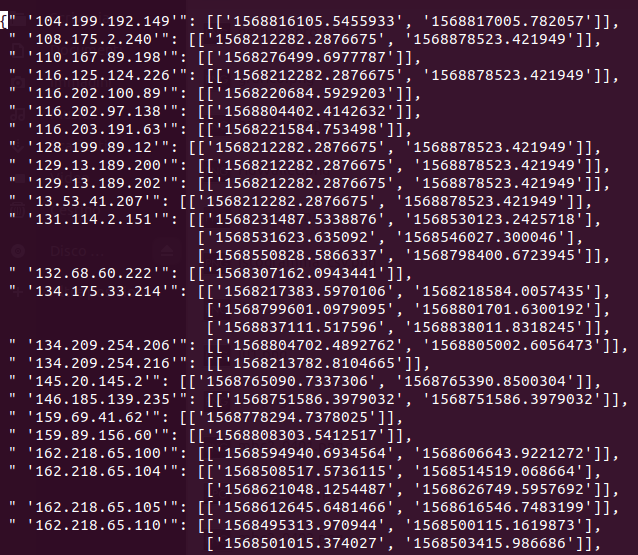
\includegraphics[width=0.755\textwidth]{imgs/intervalli.png}
   \caption{Intervalli di connessione per ogni \textit{peer}}
   \end{center}
   \hfill
\end{figure}




\section{Risultati ottenuti} 
In questo esperimento abbiamo raccolto dati per 10 giorni dal \textit{ 2019-09-11 16:31:22} al \textit{2019-09-19 09:35:23}. Ecco espessi in tabella alcuni risultati che abbiamo ottenuto:

\begin{table}[h!]
    \label{tab:table1}
    \scalebox{1}{
    \begin{tabular}{c|c|c|c|c|c} % <-- Alignments: 1st column left, 2nd middle and 3rd right, with vertical lines in between
      \textbf{Numero Lanci} & \textbf{media peer} & \textbf{varianza} & \textbf{\% nodi invariati} & \textbf{peer conosciuti}\\
      \hline
      2220  & 23.767 &0.218 & 70.1 &196 \\
    \end{tabular}
    }
\end{table}


\begin{table}[h!]
    \label{tab:table1}
    \scalebox{1}{
    \begin{tabular}{c|c|c|c} % <-- Alignments: 1st column left, 2nd middle and 3rd right, with vertical lines in between
      \textbf{max connessioni} & \textbf{nr. max connessioni} & \textbf{min connessioni} & \textbf{nr. min connessioni}\\
      \hline
      24 & 1748 & 22& 43\\
    \end{tabular}
    }
\end{table}
Sappiamo che il protocollo Bitcoin cerca di stabilire per ogni \textit{peer} 24 connessioni con altri nodi per renderlo "ben connesso". Da questi dati vediamo che, per quanto riguarda la nostra analisi, la media delle connessioni si aggira ad un numero molto vicino a 24 e inoltre osservando che la varianza ha un valore basso possiamo dire che in generale il numero di connessioni rimane sempre vicino al 24.\\
Non si \`e mai verificato un caso in cui si \`e superato questo numero di connessioni in un dato istante, ma invece questo \`e stato il massimo valore registrato dal nostro programma, mentre il minimo \`e stato 22, che da appunto conferma, come la varianza, che il numero di connessioni resta sempre "quasi" costante. La maggiorparte delle monitorizzazioni (con precisione 1748/2220) mostrano che il numero di connessioni che Bitcoin cerca di mantenere per ogni nodo \`e esattamente 24.
Il numero di peer per\`o con cui siamo venuti in contatto \`e 196, quindi significa che pi\`u volte delle connessioni sono "crollate" e se ne sono stabilite delle nuove.
Dal grafico a barre riportato dal programma, \`e possibile analizzare la percentuale del tempo totale di connessione per ogni \textit{peer} con il nostro \textit{full-node}. Riportiamo qui solamente i dati che pi\`u ci interessano:\\\\
\begin{table}[h!]
    \label{tab:table1}
    \scalebox{0.8}{
    \begin{tabular}{l|c|c|c|c|r} % <-- Alignments: 1st column left, 2nd middle and 3rd right, with vertical lines in between
      \textbf{media prob. peer} & \textbf{varianza} & \textbf{\% min. connessione} & \textbf{nr. nodi con \% minima} & \textbf{nr. nodi stabili} &\\
      \hline
       0.878 & 0.083 & 0.045\% & 43 & 14 \\
    \end{tabular}
    }
\end{table}
\\non conoscendo come si comporta il protocollo Bitcoin riguardo la topologia della rete, e quindi non sapendo se ci possano essere connessioni con alcuni \textit{peer} pi\`u probabili di altre, abbiamo dato ad ogni \textit{peer} incontrato una probabilit\`a di connettersi al nostro \textit{full-node} a seconda di quante volte \`e stato "incontrato" in passato.
Il primo valore della tabella indica la media di queste probabilit\`a con accanto la relativa varianza, ma questo potrebbe anche non essere quindi un dato che rispecchi effettivamente l'andamento delle cose nel protocollo Bitcoin.
Viene riportato inoltre nella tabella la percentuale minima della connessione di un nodo durante la monitorizzazione. Questa percentuale \`e molto bassa e come vediamo sono ben 43 i nodi che hanno il medesimo valore, questo pu\`o star a significare che c'\`e stato bisogno pi\`u volte di cambiare connessione prima di trovare un nodo pi\`u "stabile". Sono invece 14 i nodi che sono rimasti sempre connessi, e questi potrebbero essere nodi "stabili" della rete, che ci assicurano una connessione all'interno al network Bitcoin e che quindi probabilmente sono necessari.
Per quanto riguarda la geolocalizzazione abbiamo ottenuto:\\
\begin{table}[h!]
    \label{tab:table1}
    \scalebox{0.8}{
    \begin{tabular}{l|c|c|c|c|r} % <-- Alignments: 1st column left, 2nd middle and 3rd right, with vertical lines in between
      \textbf{continente max} & \textbf{stato max} & \textbf{citt\`a max} & \textbf{continente min} & \textbf{stato min} \textbf{citt\`a min}\\
      \hline
      North America & United States & Tigar & Asia & Austria & Linz\\
        153 & 153 & 109 & 18 & 1 & 1\\ 
    \end{tabular}
    }
\end{table}
\\Dove i campi indicano i luoghi e il numero (massimo e minimo ) di peer di cui siamo venuti a conoscenza, rispettivamente per continente, stato e citt\`a.
La maggior parte dei \textit{peer} che abbiamo incontrato, che ricordiamo erano 196, vengono dal nord america, e di questi tutti sono statunitensi, quindi precisamente il 78\% dei \textit{peer} sono americani. Questo potrebbe voler dire che questo \`e il luogo dove la tecnologia si \`e diffusa maggiormente?
In ultimo luogo vogliamo vedere se \`e possibile che un qualche nodo che si disconnette dal nostro \textit{full-node} sia propenso, o almeno ci sia qualche probabili\`a che possa ristabilire una connessione.
Come mostato dai dati ricavati dal nostro programma di analisi, vediamo che questa situazione capita non di rado, mostriamo gli intervalli di tempo (rappresentiamo i timestamp) di alcuni peer per cui si \`e vefiricato questo fatto:

\begin{table}[h!]
    \label{tab:table1}
    \scalebox{0.7}{
    \begin{tabular}{c|c|c} % <-- Alignments: 1st column left, 2nd middle and 3rd right, with vertical lines in between
      \textbf{131.114.2.151} & \textbf{162.218.65.241} & \textbf{23.92.36.28} \\
      \hline
      (1568231487.5338876, 1568530123.2425718) & (1568540025.947396, 1568543326.6773708) & (1568584437.7690363, 1568586538.3642185)\\ 
        (1568531623.635092, 1568546027.300046) & (1568668761.6218576, 1568668761.6218576) & (1568587138.5555046, 1568595540.8496878)\\
         (1568550828.5866337, 1568798400.6723945) & (1568669961.9677079, 1568673563.005906)\\ 
    \end{tabular}
    }
\end{table}
 
 
  











